	%%%%%%%%%%%%%%%%%%%%%%%%%%%%%%%%%%%%%%%%%
% License:
% CC BY-NC-SA 3.0 (http://creativecommons.org/licenses/by-nc-sa/3.0/)
%Blue is too flat.
%Too much content.
%simple and to the point.
% 3 introductory slides fine.
%Keep all font big, including title and bibliography page.

%'Du-nor "Jun orh'
%%%%%%%%%%%%%%%%%%%%%%%%%%%%%%%%%%%%%%%%%

%----------------------------------------------------------------------------------------
%	PACKAGES AND THEMES
%----------------------------------------------------------------------------------------

\documentclass{beamer}

\mode<presentation> {

%\usetheme{default}
%\usetheme{AnnArbor}
%\usetheme{Antibes}
%\usetheme{Bergen}
%\usetheme{Berkeley}
%\usetheme{Berlin}
%\usetheme{Boadilla}
%\usetheme{CambridgeUS}
%\usetheme{Copenhagen}
%\usetheme{Darmstadt}
%\usetheme{Dresden}
%\usetheme{Frankfurt}
%\usetheme{Goettingen}
%\usetheme{Hannover}
%\usetheme{Ilmenau}
%\usetheme{JuanLesPins}
%\usetheme{Luebeck}
\usetheme{Madrid}
%\usetheme{Malmoe}
%\usetheme{Marburg}
%\usetheme{Montpellier}
%\usetheme{PaloAlto}
%\usetheme{Pittsburgh}
%\usetheme{Rochester}
%\usetheme{Singapore}
%\usetheme{Szeged}
%\usetheme{Warsaw}

% As well as themes, the Beamer class has a number of color themes
% for any slide theme. Uncomment each of these in turn to see how it
% changes the colors of your current slide theme.

%\usecolortheme{albatross}
%\usecolortheme{beaver} Good.
%\usecolortheme{beetle}
%\usecolortheme{crane} Ok.
%\usecolortheme{dolphin}Good
%\usecolortheme{dove}Basically default
%\usecolortheme{fly}awefull
%\usecolortheme{lily}Basically default
\usecolortheme{orchid}
%\usecolortheme{rose}
%\usecolortheme{seagull}
%\usecolortheme{seahorse}
%\usecolortheme{whale}
%\usecolortheme{wolverine}

%\setbeamertemplate{footline} % To remove the footer line in all slides uncomment this line
\setbeamertemplate{footline}[page number] % To replace the footer line in all slides with a simple slide count uncomment this line

\setbeamertemplate{navigation symbols}{} % To remove the navigation symbols from the bottom of all slides uncomment this line
}
\usepackage[export]{adjustbox}

\usepackage{graphicx} % Allows including images
\usepackage{booktabs} % Allows the use of \toprule, \midrule and \bottomrule in tables
%\usepackage{pgfpages}

%Adding presentation notes wrecks havoc on the document.
%\setbeameroption{show notes}
%\setbeameroption{show notes on second screen=right}
\usepackage{verbatim}
%\usepackage{pstricks-add}
\usepackage{tikz}
\usetikzlibrary{automata,positioning}
\usepackage{listings}
\usepackage{color}

\definecolor{mygreen}{rgb}{0,0.6,0}
\definecolor{mygray}{rgb}{0.5,0.5,0.5}
\definecolor{mymauve}{rgb}{0.58,0,0.82}

\lstset{ %
  backgroundcolor=\color{white},   % choose the background color; you must add \usepackage{color} or \usepackage{xcolor}
  basicstyle=\footnotesize,        % the size of the fonts that are used for the code
  breakatwhitespace=false,         % sets if automatic breaks should only happen at whitespace
  breaklines=true,                 % sets automatic line breaking
  captionpos=b,                    % sets the caption-position to bottom
  commentstyle=\color{mygreen},    % comment style
  deletekeywords={...},            % if you want to delete keywords from the given language
  escapeinside={\%*}{*)},          % if you want to add LaTeX within your code
  extendedchars=true,              % lets you use non-ASCII characters; for 8-bits encodings only, does not work with UTF-8
  frame=single,                    % adds a frame around the code
  keepspaces=true,                 % keeps spaces in text, useful for keeping indentation of code (possibly needs columns=flexible)
  keywordstyle=\color{blue},       % keyword style
  language=C,                 % the language of the code
  morekeywords={*,...},            % if you want to add more keywords to the set
  numbers=left,                    % where to put the line-numbers; possible values are (none, left, right)
  numbersep=5pt,                   % how far the line-numbers are from the code
  numberstyle=\tiny\color{mygray}, % the style that is used for the line-numbers
  rulecolor=\color{black},         % if not set, the frame-color may be changed on line-breaks within not-black text (e.g. comments (green here))
  showspaces=false,                % show spaces everywhere adding particular underscores; it overrides 'showstringspaces'
  showstringspaces=false,          % underline spaces within strings only
  showtabs=false,                  % show tabs within strings adding particular underscores
  stepnumber=2,                    % the step between two line-numbers. If it's 1, each line will be numbered
  stringstyle=\color{mymauve},     % string literal style
  tabsize=2,                       % sets default tabsize to 2 spaces
  title=\lstname                   % show the filename of files included with \lstinputlisting; also try caption instead of title
}

%\beamerdefaultoverlayspecification{<+->}
%----------------------------------------------------------------------------------------
%	TITLE PAGE
%----------------------------------------------------------------------------------------


%make title manually and then make the text white manually.	
%\title{\textcolor{white}\huge{{Why Information Flow Is Important To Digitally Reconstructed Neural Networks}}} 

%\title{\textcolor{white}\huge{{How To Detect Direction of Information Flow between neurons}}} 
\title{\textcolor{white}\huge{{Parallel Collision Detection Over Multi Compartment Morphologies in Python}}} 
%\title{\textcolor{white}\huge{{Information Transfer of Inhibitory Post Synaptic Potentials}}} 

\author{\textcolor{white}{\textbf{\Large{{R.~Jarvis \and Supervisor P.~Junor}}}}}


%mappingtheen.jpg

\institute{\textcolor{white}{\textbf{\Large{Department of Electronic Engineering \\
La Trobe University}}}}


\date{ELE5MPB Presentation, 2014}

\date{\textcolor{white}{\textbf{\Large{\today}}}} % Date, can be changed to a custom date

%\date{\fontsize{8pt}{8t}
%\textcolor{white}{http://medicalxpress.com/news/2013-11-entire-brain-brainbow-ii-technology.html}}

\setbeamertemplate{background canvas}{

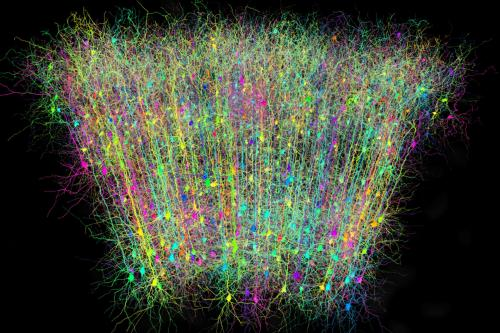
\includegraphics[width=\paperwidth,height=\paperheight]{mappingtheen.jpg}
}

%
\includegraphics[width=\paperwidth,height=\paperheight]{logo.png}
\begin{document}

\begin{frame}






\titlepage % Print the title page as the first slide


%\note<1-2>[item]{How long the presentation goes 10 minutes.}
%\note<1-2>[item]{Hello I am Russell Jarvis, my Supervisor is Paul Junor, and the title of my talk is Information flow in a digitally reconstructed neural network.}
\end{frame}

%\begin{frame}
%\note<1-2>[item]{This thesis is divided into two sections The first half concerns the background of the project and the design of the digitally reconstructed network. The second half concerns the analysis of the behaviour of the reconstructed network.}
\setbeamertemplate{background canvas}{

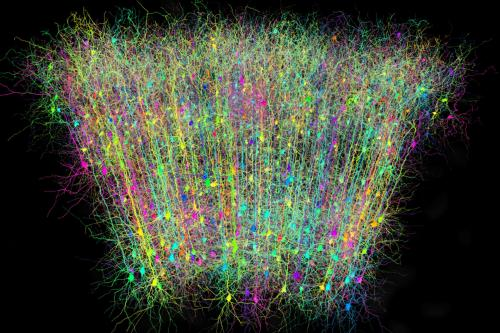
\includegraphics[width=\paperwidth,height=\paperheight]{mappingtheen.jpg}

}
%\frametitle{Overview} % Table of contents slide, comment this block out to remove it
%\fontsize{14pt}{14pt}
%\tableofcontents % Throughout your presentation, if you choose to use \section{} and \subsection{} commands, these will automatically be printed on this slide as an overview of your presentation


%\end{frame}
\setbeamertemplate{background canvas}[default] % resets the background

%----------------------------------------------------------------------------------------
%	PRESENTATION SLIDES
%----------------------------------------------------------------------------------------

%------------------------------------------------
\section{A digitally Reconstructed Network} % Sections can be created in order to organize your presentation into discrete blocks, all sections and subsections are automatically printed in the table of contents as an overview of the talk
%------------------------------------------------


\subsection{Introduction}%{Applications} % A subsection can be created just before a set of slides with a common theme to further break down your presentation into chunks

%\begin{frame}
%\frametitle{Introduction}%{Reconstructed Cortical Neural Network.}
%\begin{itemize}
%\vfill\item 
%\vfill\item There is a lot of progress in understanding information processing of sensory and motor neurons, the inputs and outputs to the brain. Information processing in cortical neural networks is much less understood. This is partly due to our ability accurately represent wiring, and reverse engineer the function of cells and networks.
\subsection{Background}%{Applications} % A subsection can be created just before a set of slides with a common theme to further break down your presentation into chunks

\begin{frame}
\frametitle{Introduction}%{Reconstruction of Networks}
\begin{itemize}
\vfill \item Made with NEURON-7.4 as a Python module. 	

\vfill \item Why did I do this, given the difficulty in staining many adjacent neurons
\vfill \item Neuromorpho data largely comes from different rodents in different labs.
\vfill \item Many of the atlas ontologies (neurons) are normalised onto one brain atlas (Allen Brain Atlas)

%\vfill\item \textbf{Reverse Engineer Principles of Brain Function:} Created a neural network model of rat cortex including accurate cell shapes. Observed information flow, making it possible to infer some functions of individual brain cells.\\

%\vfill \item Made with NEURON-7.4 as a Python module. 	
%\vfill\item I have created such a model.
%\center{\textbf{$\rightarrow$}}	
%\draw[arrows=<->](1.643,1.853)--(1.643,.12);
\begin{figure}
\centering
\begin{minipage}{.45\textwidth}
\centering
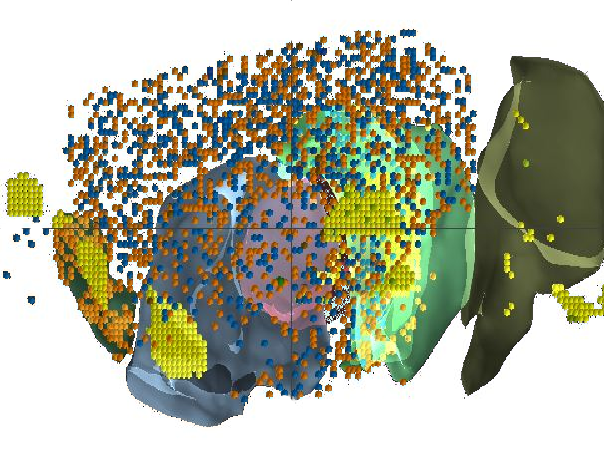
\includegraphics[scale=0.33]{pasted34.png} 
\vfill$100mm^{3}$
\end{minipage}
\begin{minipage}{.45\textwidth}
\centering
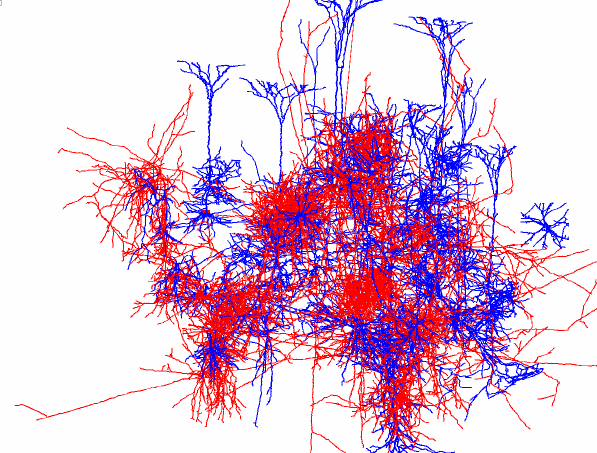
\includegraphics[scale=0.33]{pasted35}
\vfill$\mu m^{3}$
\end{minipage}
\vfill
\end{figure}

	
%\begin{figure}
%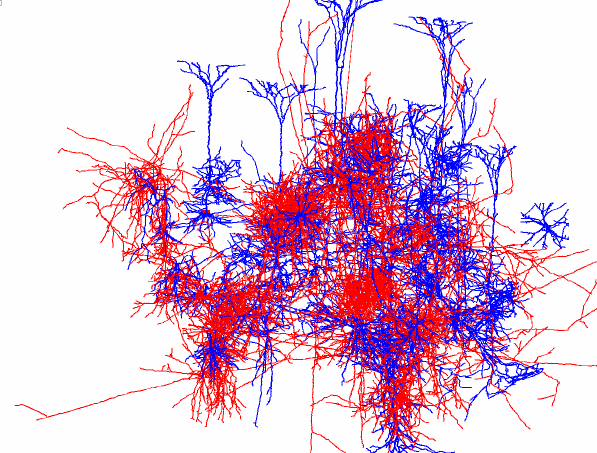
\includegraphics[scale=0.2]{pasted35} 
%\end{figure}
%\textdownarrow{}
%\downarrow

%\begin{figure}
%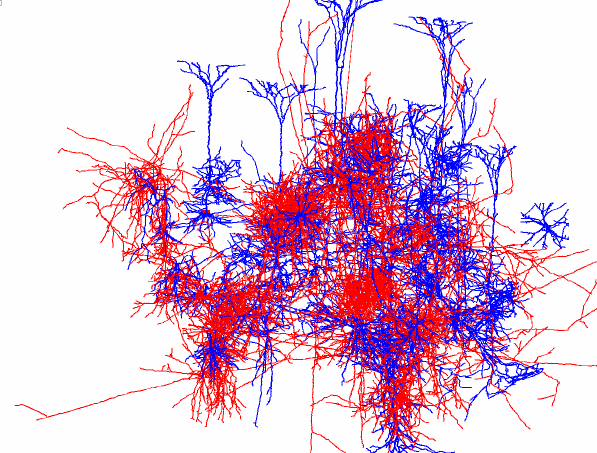
\includegraphics[scale=0.2]{pasted35}
%\caption{A volume plot of reconstructed network with membrane type classified by color} 
%\end{figure}


%\vfill \item Inferring neuron function is difficult, because one neuron can participate in different networks at different times, and neurons do not always have only one segregated function.

%\vfill \item Synapses are not resolved by light imaging of stained cells, so the network connectivity will have to be infered by the gaps between cells.

\end{itemize}
\fontsize{6pt}{6pt}\selectfont $http://neuromorpho.org/neuroMorpho/LS_Video.jsp$
\end{frame}

%\end{itemize}
%\end{frame}


%\subsection{Introduction}%{Applications} % A subsection can be created just before a set of slides with a common theme to further break down your presentation into chunks


\begin{frame}
\frametitle{Motivation}%{Reconstruction of Networks}
\begin{itemize}

\vfill \item Light Sheet microscopy, brainbow, and STED may make it possible to digitally recreate more complete forests as opposed to trees.
\vfill\item Why did I do this? I was inspired by the Blue Brain Project to find out more about real neural networks.
\vfill\item The Neuromorpho morphologies where/are temporary place holders NeuroMAC is currently able to grow realistic 3D neuron forests in silico, using a forest shapes the trees approach to neural dev.
\vfill\item Previously Ascoli's L-NAEURON has created a similar tool to grow neurons statistically form is not forest dependant.
\vfill\item Some models simply distribute Ascoli's in-silico grown trees contiguously in a line on a plane
\vfill\item Should cortical raster plots have high or low $ C_{V} $ Chaotic spike trains, may mean that the system has no memory. Regular periodic spike trains may not produce enough unique temporal patterns to be said to be temporal coding.
\end{itemize}
\end{frame}
\begin{frame}
\frametitle{Motivation}%{Reconstruction of Networks}
\begin{itemize}

\vfill\item Spike Distance, graphically showed the $C_{V}$ as the network activity proceeded through time. 
\vfill\item At the time I thought that what I was doing couldn't be any worse than the small world network topologies assumed by other models.
\vfill\item I wanted to explore issues such as location dependence of EPSPs, multiplexed rate and temporal codes but instead I looked at simpler questions.
\vfill\item Networks composed of multicompartment models exhibit much more signal selectivity can involve dendritic subunits can be excited and learn indipendantly.
\vfill\item Allen Brain has recently acquired gene expression based connectivity maps that may map to selected to the coordinates comprised by SWC files.
\end{itemize}
\end{frame}



\begin{frame}
\frametitle{Pre and Post Synapses}%{Reconstruction of Networks}
\begin{itemize}

\vfill\item In most what follows I will be referring to pre synaptic locations and post synaptic locations.
\vfill
%\begin{figure} 
%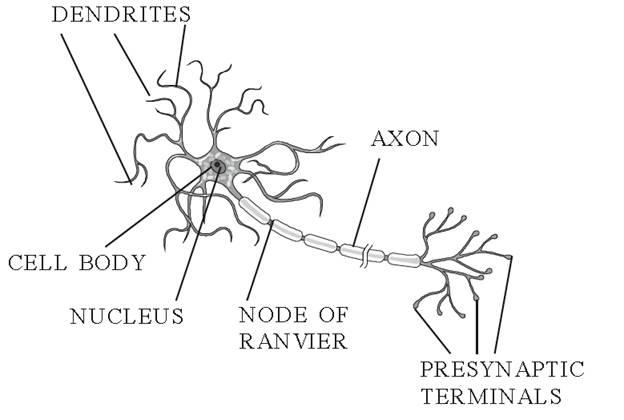
\includegraphics[scale=0.2]{anatomy1}
%	\end{figure} 

\begin{figure}
\centering
\begin{minipage}{.45\textwidth}
\centering
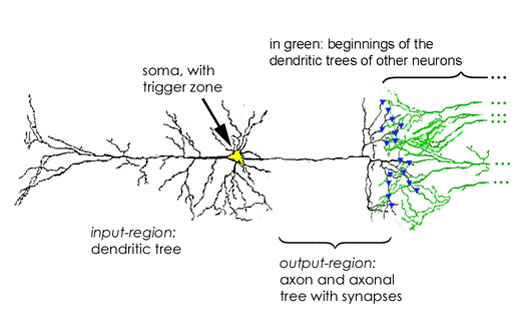
\includegraphics[scale=1.3]{ios.jpg}
\end{minipage}\hfill\hfill\hfill
\begin{minipage}{.45\textwidth}
\centering
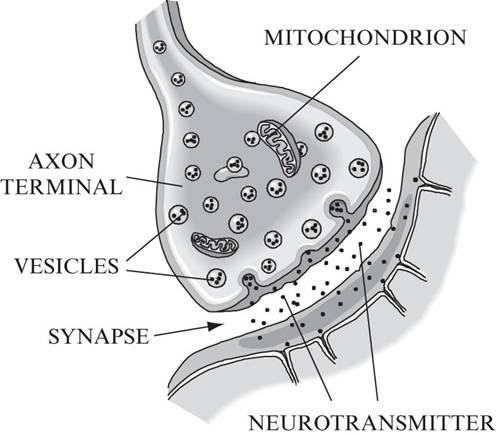
\includegraphics[scale=0.35]{anatomy2}

\end{minipage}
\vfill
\end{figure}

\end{itemize}
\vfill
\fontsize{6pt}{6pt}\selectfont 
(sources:)
http://www.igi.tugraz.at/maass/129/129a.htm

\end{frame}

\begin{frame}
\frametitle{EPSP and IPSP}
\begin{itemize}

\item \vfill Some people think of neurons as analog input digital output. %This is a simplification but an okay learning aid. The spike is the digital output
\vfill

\item \vfill One or more IPSPs can prevent a spike from occurring, by depressing the membrane potential.

\end{itemize}

\begin{figure}
\begin{minipage}{0.45\linewidth}
\centering
\includegraphics[scale=0.32]{epsp1a.jpg} 
%\caption{default}
%\label{fig:figure1}
\end{minipage}

\begin{minipage}{0.45\linewidth}
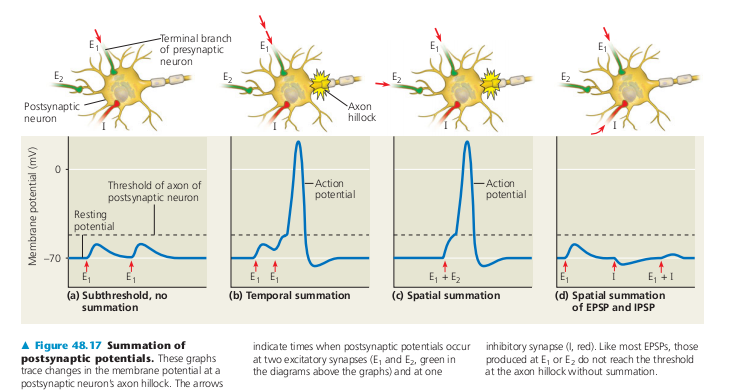
\includegraphics[scale=0.32,center]{IPSPepsp.png}

\end{minipage}
\end{figure}

%\begin{figure}
%\begin{minipage}{0.45\linewidth}
%\centering
%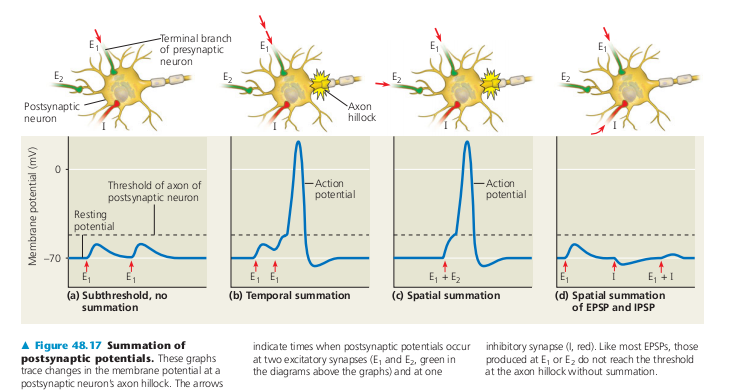
\includegraphics[scale=0.24]{IPSPepsp.png} 

%\end{minipage}
%\begin{minipage}{0.45\linewidth}
%\centering
%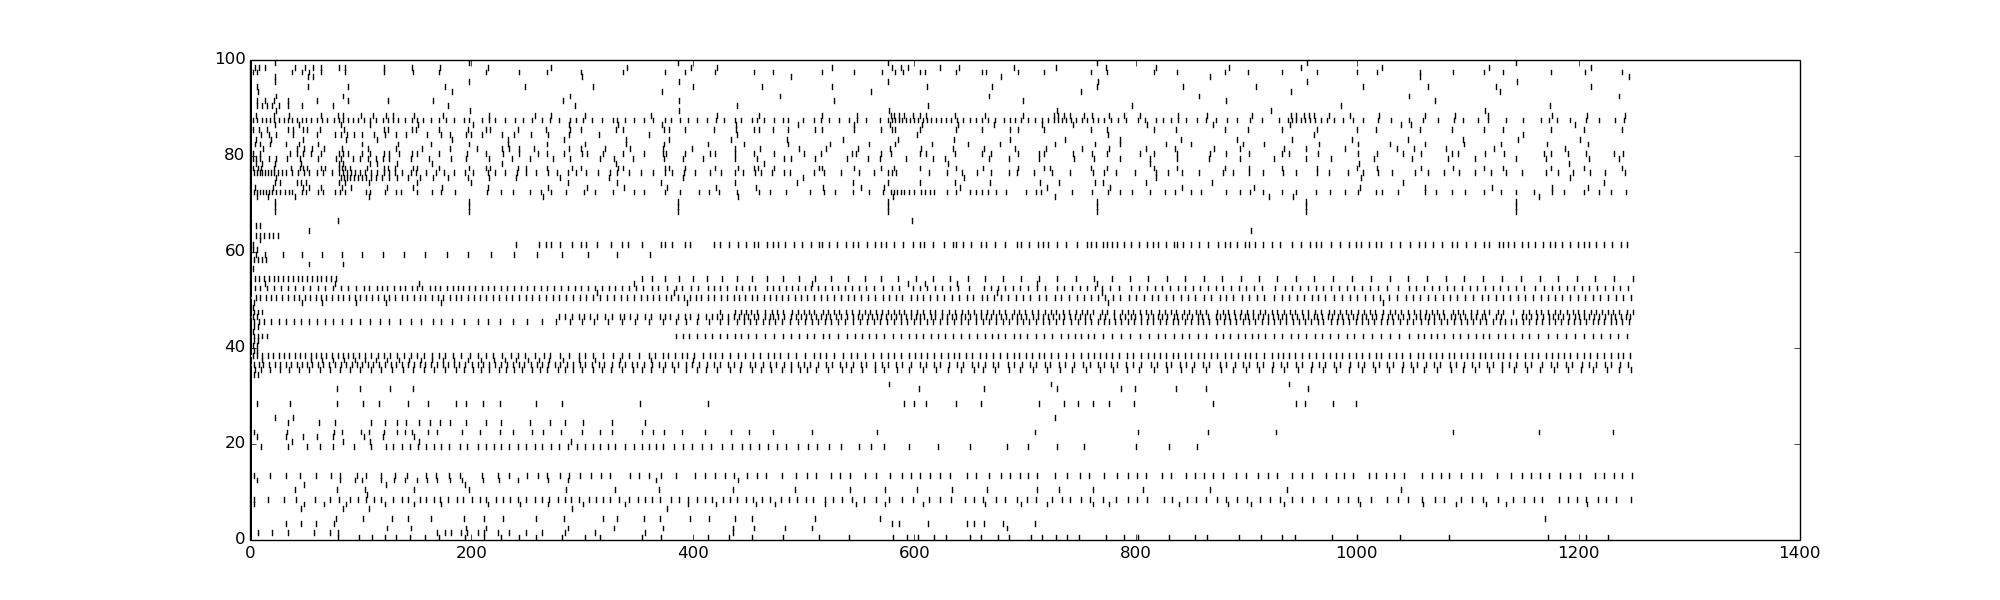
\includegraphics[scale=0.13]{raster.png}

%\end{minipage}
%\end{figure}
\vfill
\fontsize{6pt}{6pt}\selectfont 
(sources:) http://www.cerebromente.org.br/n12/fundamentos/neurotransmissores/neurotransmitters2.html

http://www.studyblue.com/notes/note/n/chapter-48-nervous-system/deck/4169450

\end{frame}





%\begin{figure}
%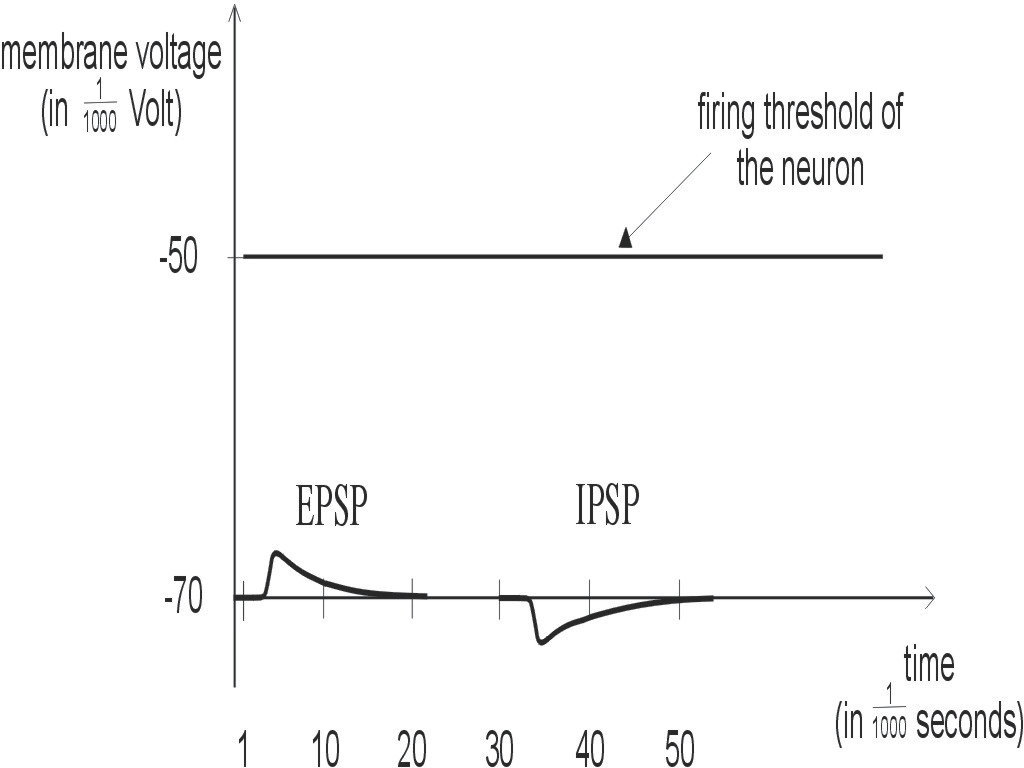
\includegraphics[scale=0.1]{ImageEPSP.png} 

%\end{figure}

%\begin{figure}
%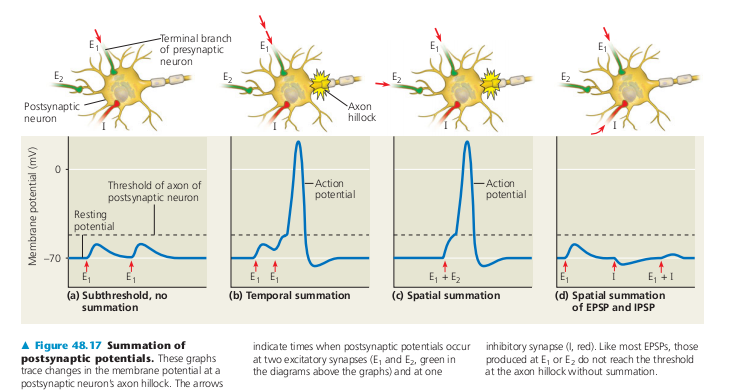
\includegraphics[scale=0.2]{IPSPepsp.png} 

%\end{figure}

%Say: both Na and K are positive ions. In the short term their flux in or out of the cell. Increases or decreases the membrane potential respectively.
%\begin{figure}
%\includegraphics[scale=0.35]{/home/zaza3/epsp1a.jpg} 

%\end{figure}

%say IPSPs cause sodium to flow out of the cell, EPSPs make sodium flow into the cell, which changes the voltage, and initiates feedback loop where voltage sensitive ion channels open. Letting more sodium in.





%\end{figure}
%\end{itemize}

%------------------------------------------------
\section{Information in the Brain}
%------------------------------------------------

\begin{frame}{Pre Processing Signals: Spike Trains}
\begin{itemize}
%\vfill \item The continuous membrane potential in a cortical neuron at any one time is partially determined by excitatory and inhibitory post synaptic potentials.

%Possibly not analog in binary out

\vfill \item Continuous membrane potential thresholded, the times each neuron fires is stored. Time binning makes signal coarse grained. % there are at least two different representations. %This is because codes employed by sensory and motor pathways, are understood to operate on the level of these discrete events.
\end{itemize}

\begin{figure}
\centering
\begin{minipage}{0.45\linewidth}
\centering
\includegraphics[scale=0.23]{pyr_nrn_memb_potential_in_degree_check0_0500_012501_00_0100_01_010_0.png}
%\caption{default}
%\label{fig:figure1}
\end{minipage}
%\hspace{0.5cm}
\begin{minipage}{0.45\linewidth}
\centering
\includegraphics[scale=0.23]{spikes_2.png}
%\includegraphics[width=\textwidth]{filename2}
%\caption{default}
%\label{fig:figure2}
\end{minipage}
\end{figure}

\begin{figure}
\begin{minipage}{0.45\linewidth}
\centering
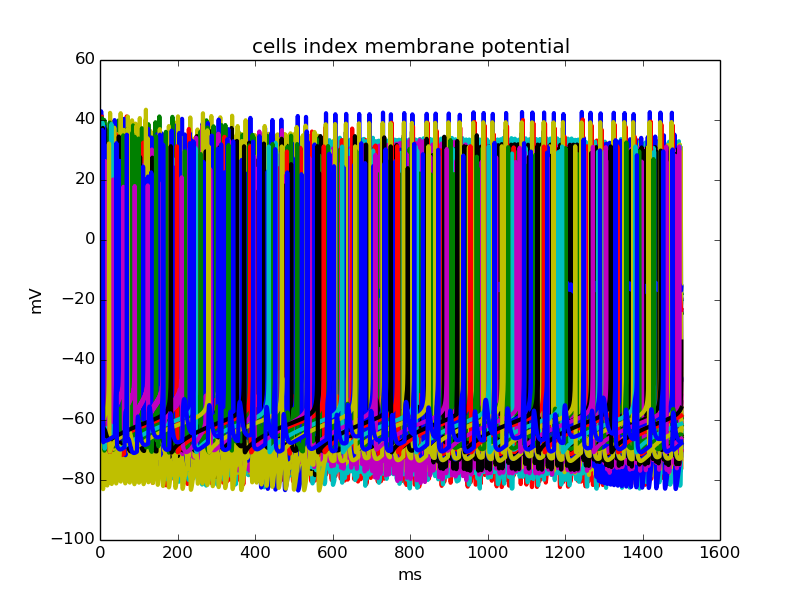
\includegraphics[scale=0.26]{allMemb.png}

\end{minipage}
\begin{minipage}{0.45\linewidth}
\centering
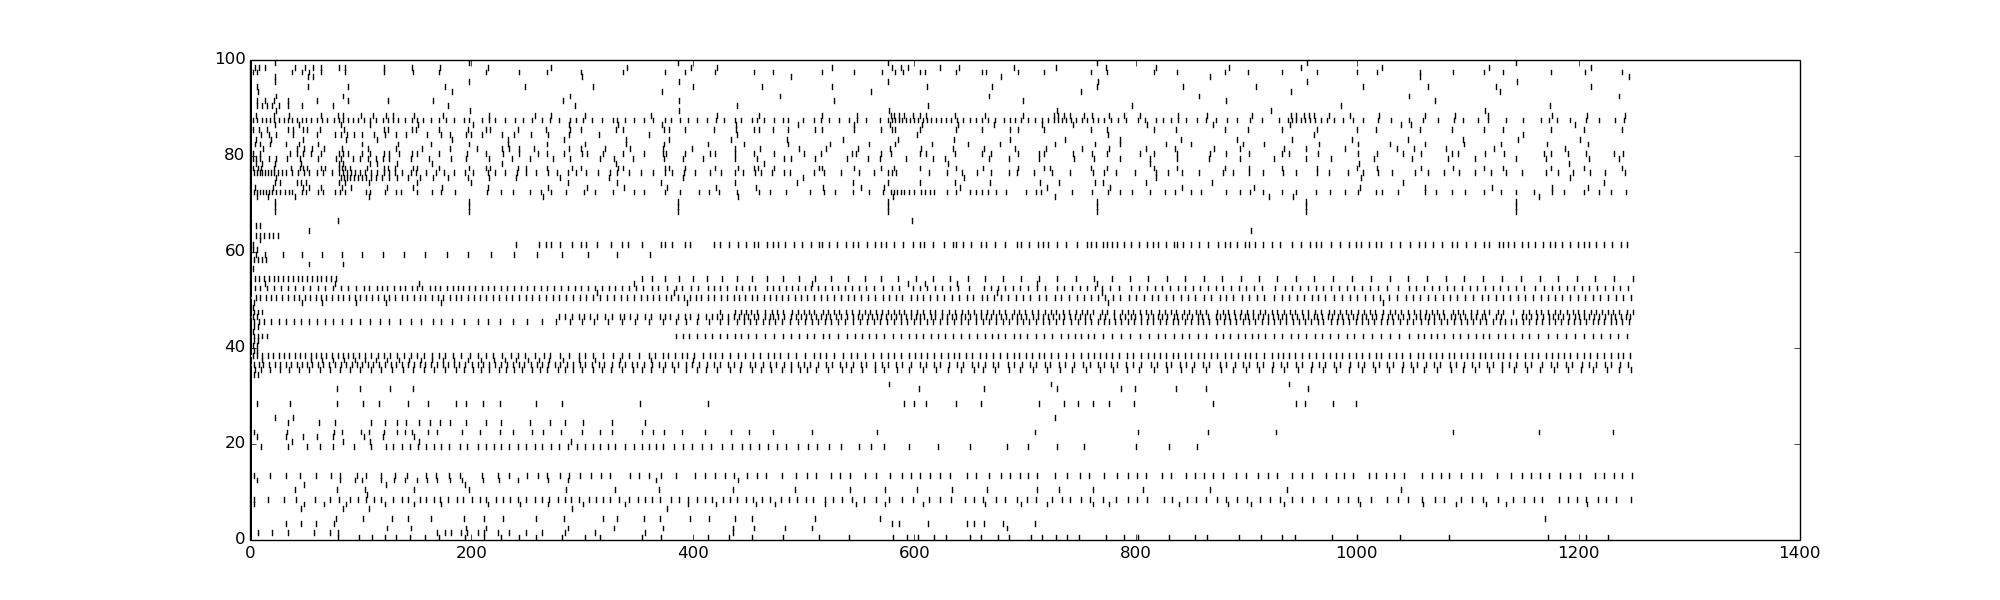
\includegraphics[width=0.9\textwidth,height=0.36\textheight]{raster.png}

\end{minipage}
\end{figure}
\end{frame}

%\begin{figure}
%\centering
%\begin{minipage}{0.45\linewidth}

%\includegraphics[scale=0.22]{/home/zaza3/graphs/20140517/pyr_nrn_memb_potential_in_degree_check0_0500_012501_00_0100_01_010_0.png}
%\caption{default}
%\label{fig:figure1}
%\end{minipage}
%\hspace{0.5cm}

%\begin{minipage}{0.45\linewidth}
%\centering

%\includegraphics[scale=0.22]{/home/zaza3/spikes_2.png}
%\includegraphics[scale=0.35]{/home/zaza3/images/spike_train.png}	
%\includegraphics[width=\textwidth]{filename2}
%\caption{default}
%\label{fig:figure2}
%\end{minipage}
%\end{figure}

%\begin{figure}
%\begin{minipage}{0.45\linewidth}
%\centering
%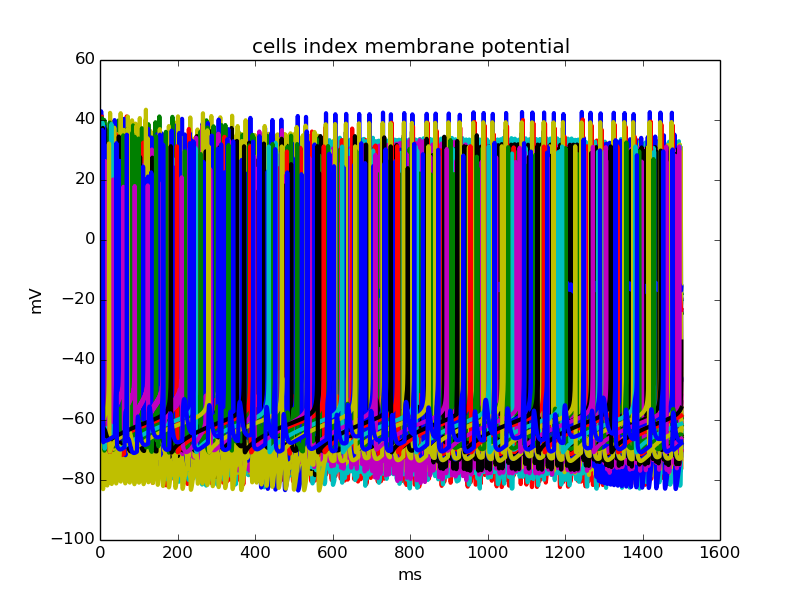
\includegraphics[scale=0.27]{allMemb.png}

%\end{minipage}
%\begin{minipage}{0.45\linewidth}
%\centering
%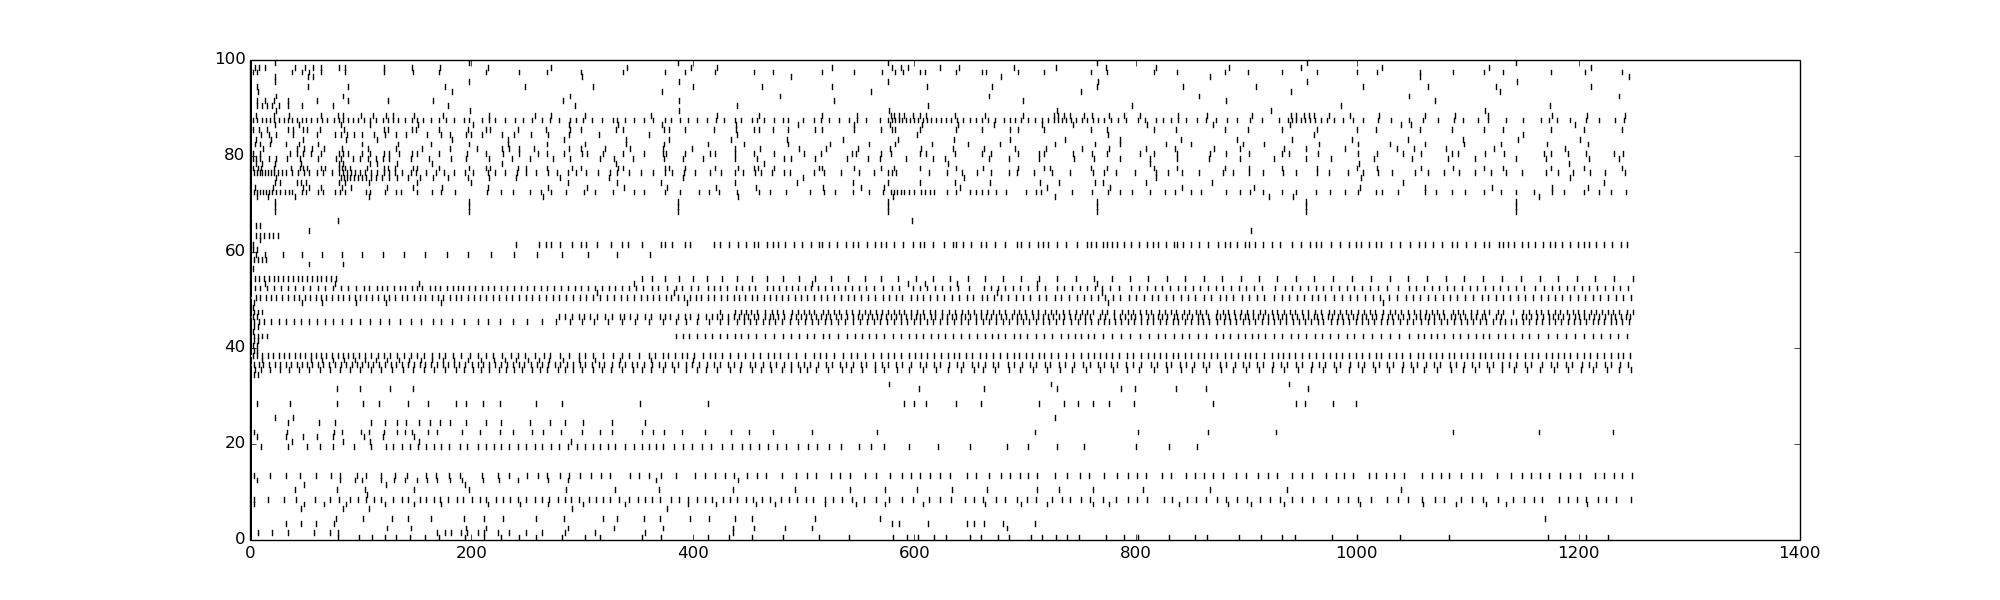
\includegraphics[scale=0.18]{raster.png}
%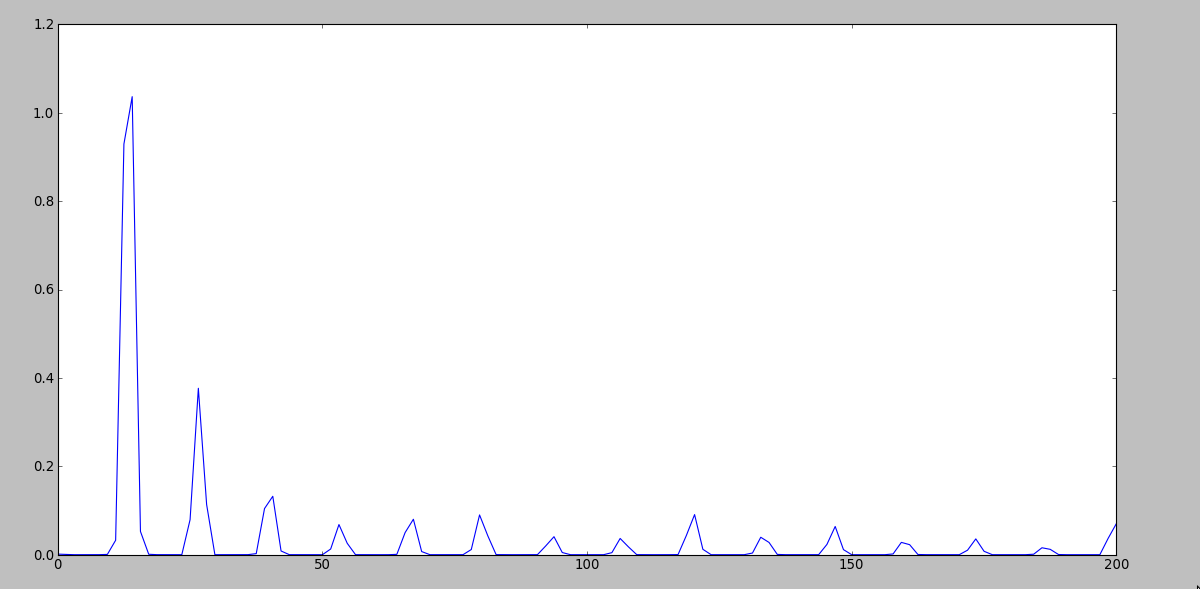
\includegraphics[scale=0.27]{pasted1}

%\end{minipage}
%\end{figure}



\subsection{Background motivation}%{Applications} % A subsection can be created just before a set of slides with a common theme to further break down your presentation into chunks



%\begin{frame}{Background motivation}
%\frametitle{Background Motivation}
%\begin{itemize}
%\vfill \item  \textbf{Reverse Engineer Principles of Brain Function:} By reconstructing in vivo neural networks in %silico
%simulation and observing information flow, it may become possible to infer neuron function.

%It is desirable to identify neurons that emit streams of stored information, and other neurons that generate working memories.

%\note<1-2>[item]{By modelling all of the detail and behavior of neural networks, it is possible to reverse engineer principles of brain function.}


%\note<1-2>[item]{Those functions can include coincidence detection, filtering, thresholding, coincidence detection, and temporal integration. The computations mentioned above described operations on information. However information transformation is caused by physical modulation of the membrane potential which occurs because of the contribution of additional computations not yet described. At the level of a single neuron membrane potential additional computations can include amplification, filtering, linear or non-linear integration, and also temporal and spatial integration. At the level of the network additional computations can include amplifying and attenuating affects caused by positive and negative feedback loops. Additionally Spike timing Dependent Plasticity can allow synapses to learn to favor certain combinations of inputs\cite{van2000stable} \cite{izhikevich2006polychronization}.\\* 

%In contrast to information provided by sensory stimulation to the network, certain properties of the network and the cells that comprise it give rise to information. I will refer to information that originates from inside the network as 'intrinsic information'. Intrinsic information can be viewed as the result of a particular type of information transformation, were new information is created by recombining two or more otherwise unaltered streams of sensory information at a neuron.\\* 


%In vivo neural networks are likely to have been optomised through evolution to perform specific computing functions. Some of these computing functions result in operations on information such as information transmission, information receiving, active information storage, and information transformation \cite{neymotin2011synaptic}. The ultimate aim of analysing this network model is to characterise the information operations sub-served by the neurons and the network.\\* }


%\vfill \item From Digitally Reconstructed neurons to Digitally reconstructed Networks.

%\lyxframeend{}
%------------------------------------------------

%------------------------------------------------


%\begin{frame}
%\frametitle{Start off with a Digitally reconstructed network.}
%A wiring algorithm searched for the coordinates of contact points and inserted a network connection.
%\begin{figure}
%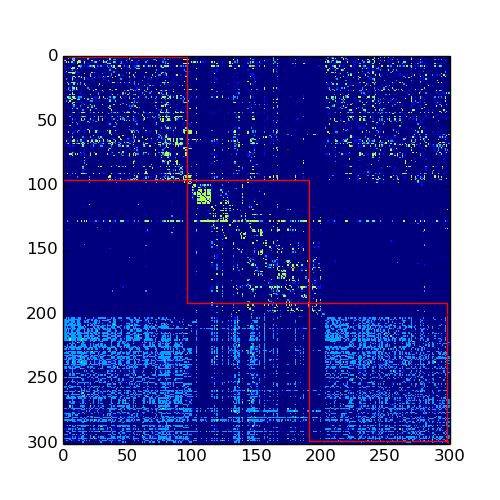
\includegraphics[scale=0.30]{expericomp/backuptex/louvain300}
%\end{figure}
%\end{frame}




\begin{frame}
\frametitle{Connectivity and the Adjacency Matrix.}



\begin{figure}
\centering
\begin{minipage}{0.45\linewidth}

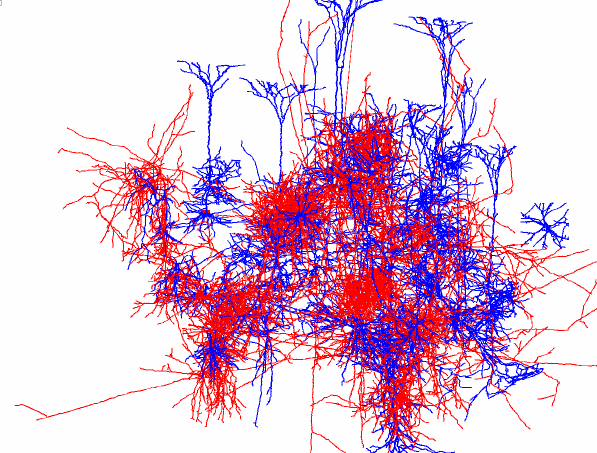
\includegraphics[scale=0.24]{pasted35}

%\caption{Volume plot 25 cells}


\end{minipage}
%\hspace{0.5cm}
\begin{minipage}{0.45\linewidth}
\centering
%\includegraphics[scale=0.24]{/home/zaza3/graphs/20140517/Both_transmitters_degree_matrix0_0500_012501_00_01009_010_0.png}
%\includegraphics[width=\textwidth]{filename2}
%\caption{default}
%\label{fig:figure2}
\end{minipage}
\end{figure}
\fontsize{8pt}{8pt}\selectfont \center{I$\rightarrow$E=2073,     $fb_{1}-=1081$}                  
%\\E$\rightarrow$E=1775 }
\begin{figure}
\begin{minipage}{0.45\linewidth}
\centering
%\includegraphics[scale=0.24]{/home/zaza3/graphs/20140517/AMPA_degree_matrix0_0500_012501_00_010011_010_0.png}
\end{minipage}
\begin{minipage}{0.45\linewidth}
\centering
%\includegraphics[scale=0.24]{/home/zaza3/graphs/20140517/GABA_degree_matrix0_0500_012501_00_010010_010_0.png}
\end{minipage}
\end{figure}

\end{frame}

%Valuable information about network connectivity extracted from the adjacency matrices, including the number of projections between populations of neurons. The number positive and negative feedback loops.
%\includegraphics[scale=0.30]{/home/zaza3/graphs/20140516/AMPA_degree_matrix0_0500_025001_00_010011_010_0.png}

%EI 1018\\ 
%II 1959\\ 
%IE 3240\\ 
%$fb_{1}-=1081$\\  
%$fb_{1}+=689$\\
%\center{EE 1775}\\ 
%EI 465\\ 
%II 1100\\ 
%IE 2073\\
\begin{frame}
\frametitle{Information In the Spike Train}
\subsection{Stored Information}
\begin{itemize}
\vfill \item The number of spikes per bin: $\Delta t$ is the source of uncertainty in the spike train.
%\vfill \item
\vfill \item There are two major sources of information: 
\vfill \item 1st the external input (sensory).
\vfill \item 2nd sources of variability that are intrinsic to the brains dynamics. 
\end{itemize}

\begin{figure}
\centering
\begin{minipage}{0.45\linewidth}
%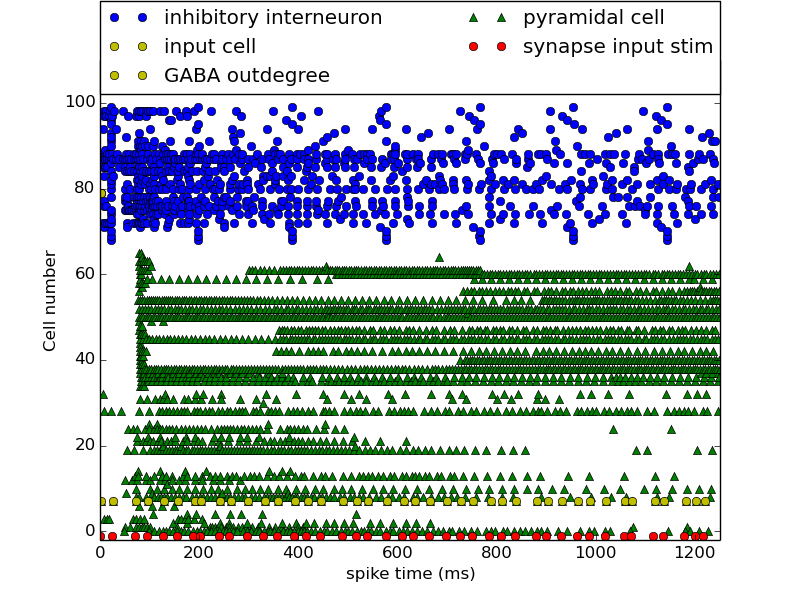
\includegraphics[scale=0.25]{raster_plot0_0500_012501_00_0100_00_010_0.png}
%\vfill
%\center{Raster Plot}
%\end{minipage}
%\centering
%\begin{minipage}{0.45\linewidth}
%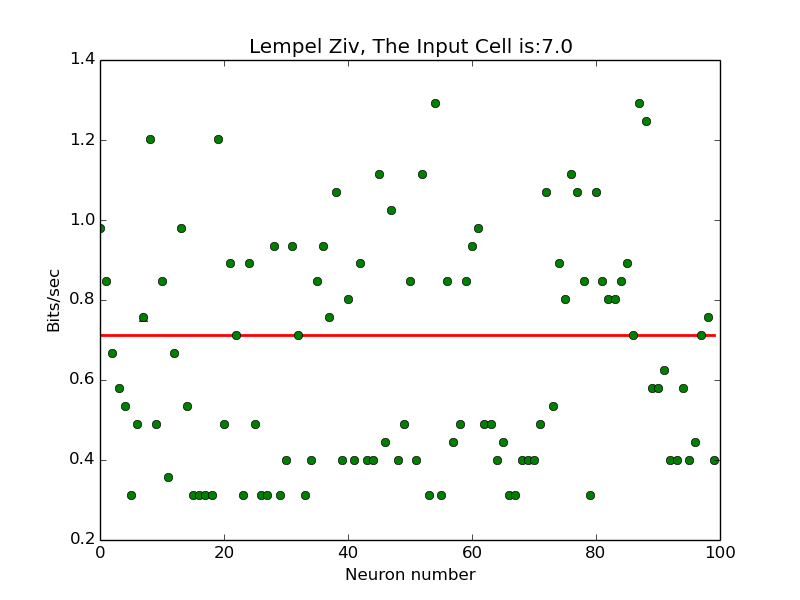
\includegraphics[scale=0.25]{Lempel_Ziv0_0500_012501_00_01006_010_0.png}
%\vfill\hfill
%\center{Lempel Ziv Complexity}
\end{minipage}
\end{figure}


\end{frame}


\begin{frame}{An Interpretation of Information Flow:Prediction}
\begin{itemize}
%\item \vfill Information is Shannon Information.\\


\item \vfill Using Transfer Entropy we can say that $neuron_{Y}$ influences $neuron_{X}$ if $neuron_{Y}$'$s$ past activity reduces the uncertainty about $neuron_{X}$'$s$ future activity. 
\begin{figure}


\centering 


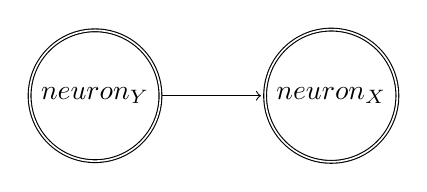
\begin{tikzpicture}[shorten >=1pt,node distance=3cm,on grid,auto]



   \node[state,accepting] (q_0)   {$neuron_{Y}$}; 
   \node[state,accepting](q_3) [right=of q_0] {$neuron_{X}$};
    \path[->] 
    (q_0) edge  node {} (q_3);
\end{tikzpicture}
\end{figure}
\item \vfill When a particular type of entropy (uncertaintity) is reduced prediction is increased.
\end{itemize}


\end{frame}



\begin{frame}{Resulting Information Flow}
\begin{itemize}

\vfill \item One cell can predict another cells activity acting through intermediate neurons%Say without direct connections 
\vfill \item A reduction in firing probability still represents an information transmission influence.
%, if cells considered have phase locked (but asynchronous) activity. Or if a time lagged spike train has similar information to a non time lagged one, just by chance.
\end{itemize}
\begin{figure}
\begin{minipage}{0.45\linewidth}
\centering
\includegraphics[scale=0.301]{Both_transmitters_degree_matrix0_0500_012501_00_01009_010_0.png}

\vfill Connectivity


\end{minipage}
\begin{minipage}{0.45\linewidth}
\centering


\includegraphics[scale=0.301]{nTE_matrix_imshow0_0500_0125010_010012_010_0.png}
\vfill nTE

\end{minipage}
\end{figure}

\end{frame}




\begin{frame}{Information Flow Between Neurons}

\section{Information Flow}
%\include{results_structure}
%\include{time_results}%extension confuses it.
%\include{pictures4lyx5}
%zaza3@zaza3:~/graphs/20140517$ eog *.png

%\begin{figure}
%\includegraphics{/home/zaza3/Documents/lempelzivcomplexity100.png}
%\end{figure}

\begin{itemize}
%s\fontsize{8pt}{8pt}\selectfont 

\vfill \item Degree matrix shows the quantity and direction of information transmitted between each pair of neurons.
%Transfer entropy is assymetrical. Correlation is symmetric.

%\vfill \item Degree matrix shows the amount of information transmitted between neurons. Transfer entropy is normalised between 0-1, so units are not bits.


%\vfill \item The matrix depicts entropy transfered from one neuron to another neuron. The matrix shows that there is enough similarity in some neuron spike trains to reduce the uncertainty about information in other neural spike trains. Thus not all the spike trains are being transformed and some of the same information is flowing through the network.

\begin{figure}
\begin{minipage}{0.45\linewidth}
\centering
\includegraphics[scale=0.301]{nTE_matrix_imshow0_0500_0125010_010012_010_0.png}
\vfill nTE

\end{minipage}
\begin{minipage}{0.45\linewidth}
\centering
\includegraphics[scale=0.301]{correlations0_0500_012501_00_010013_010_0.png}
\vfill Correlation Matrix

\end{minipage}
\end{figure}

%\end{frame}

%\begin{figure}

%\includegraphics[scale=0.25]{/home/zaza3/graphs/20140517/nTE_matrix_imshow0_0500_0125010_010012_010_0.png}

%\end{figure}

%\begin{figure}
%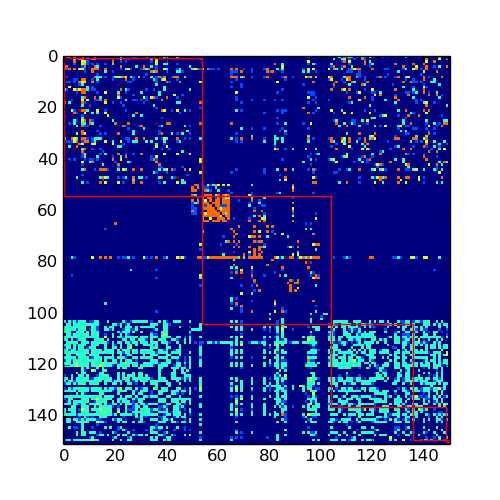
\includegraphics[scale=0.30]{/home/zaza3/expericomp/backuptex/community_partitions150cells.png}
%\includegraphics[scale=0.25]{/home/zaza3/graphs/20140517/correlations0_0500_012501_00_010013_010_0.png}
%\end{figure}



\vfill \item Presence of information flow contributes  validation of reconstruction because when information does flow, it suggests information is not randomly created and destroyed at every node.

%\vfill \item The matrix is used to observe information flowing through the network. If the type of information in different parts of the network is related or similar, that will help to validate the network, since it will no longer be randomly transforming the information.

%\vfill \item Check to see if there is a stream of stored information that is merging with the external stream of information that was used to stimulate the network.
\end{itemize}

\end{frame}
%\includegraphics[scale=0.25]{/home/zaza3/graphs/20140517/nTE_matrix_imshow0_0500_0150010_08512_010_0.png}





\begin{frame}
\frametitle{Information Flow}
\subsection{Information Flow}
\begin{itemize}
\vfill \item In Von Neuman architecture no conflict between transmitting, translating, and storing information. %Such a conflict is avoided by performing those operations on different dedicated electronic components. 
Respective tasks performed by the bus, the CPU, RAM. One entire neuron simultaneously engages in information transfer, information alteration and information storage. 
\end{itemize}
%\vfill \item The matrix depicts entropy transfered from one neuron to another neuron. The matrix shows that there is enough similarity in some neuron spike trains to reduce the uncertainty about other neural spike trains. Thus not all the spike trains are being randomly transformed and information is flowing through the network.
%\begin{figure}
%\begin{minipage}{0.45\linewidth}
%\centering
%\includegraphics[scale=0.19]{/home/zaza3/graphs/20140517/%nTE_matrix_imshow0_0500_0125010_010012_010_0.png}
%\includegraphics[width=\textwidth]{filename2}
%\caption{default}
%\label{fig:figure2}
%\end{minipage}
%\end{figure}

\begin{figure}
\begin{minipage}{0.495\linewidth}
\centering
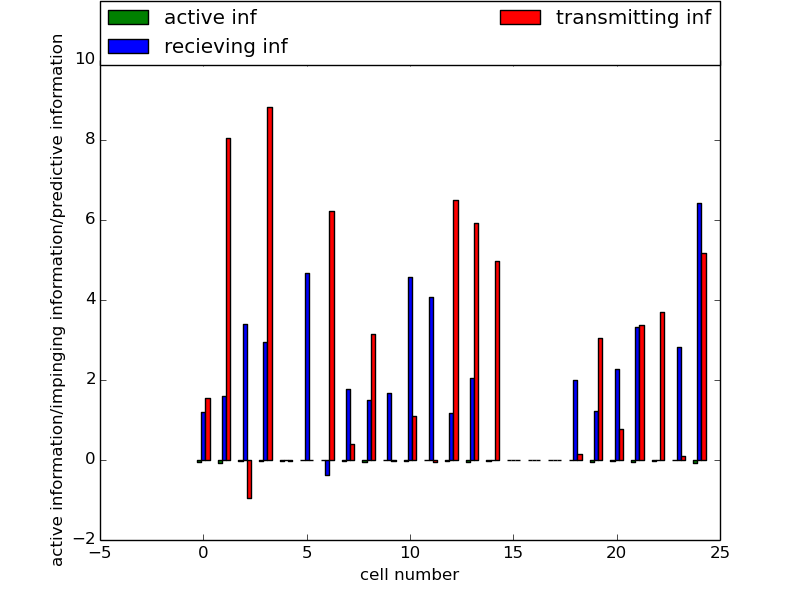
\includegraphics[scale=0.29]{Active_impinging_predictive10_012501_00_010022_010_0.png}
%\vfill Sum of Matrix Elements 
\vfill Sums, Cells[0,24]
\end{minipage}
\begin{minipage}{0.495\linewidth}
\centering
\includegraphics[scale=0.29]{Active_impinging_predictive20_012501_00_010022_010_0.png}%Active_impinging_predictive10_012501_00_010022_010_0.png}
%\vfill Sum of Matrix Elements 
\vfill Sums, Cells[25,49]
\end{minipage}
\end{figure}
\end{frame}

%/home/zaza3/graphs/20140517/Active_impinging_predictive30_012501_00_010022_010_0.png
%\begin{figure}

%\includegraphics[scale=0.1]{/home/zaza3/graphs/20140517/nTE_matrix_imshow0_0500_0125010_010012_010_0.png}
%\end{figure}
%\includegraphics[scale=0.25]{/home/zaza3/graphs/20140517/nTE_matrix_imshow0_0500_0150010_08512_010_0.png}


%\begin{figure}
%\includegraphics[scale=0.1]{/home/zaza3/graphs/20140517/Active_impinging_predictive10_012501_00_010022_010_0.png}
%\end{figure}

%\begin{figure}
%\includegraphics[scale=0.1]{/home/zaza3/graphs/20140517/Active_impinging_predictive10_012501_00_010022_010_0.png}
%\end{figure}

%\item An analysis of information flow in the resulting reconstructed network was performed to check each neurons information rates.

%\item To check how well the information in one cells activity can %predict 
%reduce the uncertainty about information in another cells activity. 






%------------------------------------------------
%The problem is from here onwards.



%\begin{frame}



%\frametitle{Why Information Flow Is Important}
%\subsection{Why Information Flow Is Important}
%\vfill \item An analysis of information flow in the resulting reconstructed network was performed to check each neurons information rates.

%\begin{itemize}

%\vfill \item Information flow within neurons 
%later turn into \notealso called local active information storage
%is important because it can be used to identify groups of neurons that are able to generate working memories.
%\end{itemize}

%\end{frame}
%-----------------


\begin{frame}
\frametitle{\textbf{Drawbacks and Future Work}}
\begin{itemize}

\vfill \item Predictive changes in spike train information may occur for reasons other than direct connectivity (effective connectivity). Such as when some cells are synchronised to another cell that has a direct connection.
%Linear is a subset of nonlinear.
%\vfill \item Because of the 2 level quantisation in the methods employed here can only detect information in the presynaptic spike. Additionally Spectral Granger Causality, can predict other types of activity.
\vfill
\textbf{Future work:}
\vfill \item Within cell transfer entropy. The model I implemented contains within cell and between cell feedback.  Working memory function of neurons can be inferred from within cell transfer entropy.

\vfill \item Completely parallelising the network. As well as a partial parallelisation (communication between CPUs), the implementation was performed by formulating the simulation as an embarrassingly parallel problem.

\vfill \item Inputing a signal into the normalised transfer entropy algorithm that has been qauntised into more than two levels, because neural network outputs are amplitude modulated signals.


\end{itemize}
\end{frame}


\begin{frame}
\frametitle{\textbf{Summary}}
\begin{itemize}


\vfill\item Discussed how TE identified functions. TE distinguished information sending neurons from information receiving neurons.%Think , and it can do more.\\

\vfill\item Transfer Entropy was used to quantify \textbf{Information Flow} within and between neurons.

\vfill \item I described how information flow in IPSPs can be detected.

\vfill\item I have discussed how the presence of information flow contributed to the validation of model. 
%\vfill\item It identified streams of stored information being recalled by the network.\\

\vfill \item Generally I have described the analysis of Information flow in a cortical neural network, and why it is of interest.


\end{itemize}
\end{frame}



%\begin{frame}

%\subsubsection{Information flow between neurons}
%\begin{itemize}

%\vfill \item Information flow is also important because it can identify neurons that emit a stream of stored information.

%\vfill \item To check how well the information in one cells activity can %predict 
%reduce the uncertainty about information in another cells activity. That is to observe information flowing through the network. If the type of information in different parts of the network is related or similar, that will help to validate the network, since it will no longer be randomly transforming the information.

%\vfill \item Check to see if there is a stream of stored information that is merging with the external stream of information that was used to stimulate the network.
%\end{itemize}

%\end{frame}



%------------------------------------------------


%------------------------------------------------

\begin{comment}
\begin{frame}[fragile] % Need to use the fragile option when verbatim is used in the slide
\frametitle{Wiring Algorithm 1}
\lstinputlisting[firstline=2183, lastline=2194]{/home/zaza3/expericomp20140421/fd.hoc}
\end{frame}
\end{comment}


%------------------------------------------------

%\begin{frame}
%\frametitle{Information Flow}
%\subsection{Information Flow}
%\begin{itemize}

%\vfill \item Provide A frame work for Classify neurons according to three operations:
%information transmission, information storage, spike train modification.
%\end{itemize}

%\vfill \item Spike train modification was assessed using Kreutz multivariate Spike
%Distance, and the coefficient of variation.
%\vfill \item Information transferal was measured with transfer entropy and Spectral
%Granger Causality


%\pause{}

%\vfill \item These overlays are created using the Pause style.
%\end{itemize}

%\end{frame}

%------------------------------------------------

%\begin{frame}[fragile] % Need to use the fragile option when verbatim is used in the slide

%\end{frame}

%------------------------------------------------


%comment. 10 slides only.




%Unlike conventional electronic elements a neuron can simultaneously perform information storage (encoding), information alteration, and information transmission in the same electronic elements.
%Classifying the role of neurons according to the ratio of information storage, information alteration, and information transmission. 
%Provide a frame work for assessing the contribution of neuron morphology to those three operations.





\begin{frame}
\nocite{*}
\frametitle{References}
\footnotesize{
\begin{thebibliography}{99} 
\fontsize{11pt}{11pt}\selectfont
\bibitem[Kerr, 2012]{p1} Kerr, Cliff C et al (2012)\newblock Electrostimulation as a prosthesis for repair of information flow in a computer model of neocortex
\newblock \emph{IEEE} 20(2), 153 -- 160.

\bibitem[Neymotin, 2011]{p1} Neymotin, Samuel A et al (2011)
\newblock Synaptic information transfer in computer models of neocortical columns
\newblock \emph{Journal of computational neuroscience} 30(1), 69 -- 84.

\bibitem[Gour{\'e}vitch, 2007]{p1} Gour{\'e}vitch, Boris and Eggermont, Jos J  (2007)		
\newblock Evaluating information transfer between auditory cortical neurons.
\newblock \emph{Journal of Neurophysiology} 97(3), 2533 -- 2543	

\bibitem[lizier2012local, 2012]{p1} Lizier, Joseph T  et al (2012)
\newblock Local measures of information storage in complex distributed computation
  \newblock \emph{Information Sciences} 208, 39--54
	  %publisher={Elsevier}

%\newblock \emph{Journal of Neurophysiology} 97(3), 2533--2543.
%\bibitem[Ascoli, 2007]{p1} Ascoli, Giorgio A and Donohue, Duncan E and Halavi, Maryam 2007
%\newblock NeuroMorpho. Org: a central resource for neuronal morphologies
%\newblock \emph{Soc Science} 27(35), 9247--9251.
%\bibitem[Sporns, 2011]{p1} Olaf Sporns 2011
%\newblock Networks of the brain
%\newblock \emph{MIT Press}.


\end{thebibliography}
}




\end{frame}


%------------------------------------------------The problem is after the bibliography
%\begin{frame}{\textbf{Summary}}
%\begin{itemize}
%\item I have described network reconstruction from reconstructed cells via introducing infering synapse location.

%\item I have described an algorithm for network wiring and what it can tell you based on synapse location.

%\end{itemize}
%\end{frame}


\begin{frame}
\vfill
\vfill
\vfill
\vfill
\vfill
\vfill
\vfill
\vfill
\vfill
\vfill
\vfill
\vfill
\vfill
\vfill
\begin{center}	
\fontsize{14pt}{14pt}\selectfont {\textbf{The End}}\end{center}
\vfill
\vfill
\vfill
\vfill
\vfill
\vfill
\vfill
\vfill
\vfill
\vfill
\vfill
\vfill
\fontsize{8pt}{8pt}\selectfont\center{made with \emph{\LaTeX}}

\end{frame}

\begin{frame}
\begin{center}
\fontsize{14pt}{14pt}\selectfont \textbf{Questions?}	
\end{center}
\end{frame}



\begin{frame}
\frametitle{Trifid}
\begin{itemize}
\vfill \item Trifid is a large Intel system and is VPAC's sixth and largest cluster. Trifid has 180 compute nodes, with a total of 2,880 cores. It has a HPL (high performance Linpack) rating is 45.9 TFLOPS. It obviously runs HPC Linux.
\vfill \item 180 nodes
2,880 cores of Intel $E5-2670$
\vfill \item 4 GB PC1600 memory per core (64 GB per node),
\vfill \item In practice could access (99GB on one node)%pmem=99000mb per host RAM
 with 6 nodes having 16 GB per core (256 GB per node)
%                 64000mb
\vfill \item This computer 4000mbRAM
\vfill \item 4 nodes will be GPU/MIC capable
FDR Infiniband.
\vfill \item CentOS 6 Linux
\vfill \item VPAC NFS for home
\vfill \item VPAC 165TB DDN S2A high performance array for work/scratch/projects (using Lustre).
% There are two types of ways of formulating parallel problems. The first way is trivially parallel problems. This was used to search for the effects of a change in one parameter. 
% The second way is more valuable. That involves increasing the capacity of the network, by distributing the cells across different CPUs.


\end{itemize}
\end{frame}

\begin{frame}
\frametitle{Trifid}
\begin{itemize}
\vfill \item I succesfully made an algorithm which could distribute the cells over over the hosts, in NEURON, I did this again in Python.

\vfill \item Parallelising the wiring diagram was non trivial. It was more complex than necessary using NEURON and MPI alone. Mpi4py has many nice features for easy point to point communication of Numpy Vectors. 


\end{itemize}
\end{frame}	

%Problem is below here.


\begin{frame}
\frametitle{Stored Information}
\subsection{Stored Information}
\begin{itemize}
\fontsize{8pt}{8pt}\selectfont 
\item stored information

\begin{figure}
\includegraphics[scale=0.25]{Lempel_Ziv0_0500_012501_00_01006_010_0.png}
\end{figure}
\begin{figure}
\includegraphics[scale=0.25]{raster_plot0_0500_012501_00_0100_00_010_0.png}
\end{figure}
\end{itemize}
\end{frame}

%------------------------------------------------

\begin{frame}
\frametitle{Applications}
\subsection{Applications}
\begin{itemize}

\vfill \item Reverse engineering principles of brain function.

\vfill \item The dynamic clamp Closed loop, real-time NEURON. Models a missing network, and Substites in the missing network behavior with electrode arrays. 

\vfill \item Cogntive neuro prosthesis. If we understand what neurons are doing in the hippocampus and prefrontal cortex it is more likely that we will be able to replace their functions in the future.
%\vfill \item Computation that exploits noise.
\vfill \item \textbf{Neuromorphic Engineering}: Noise tolerant AI, by using brain principles, such as computation with noise, using spiking neural networks. 
 
\vfill \item Epilepsy seizure detection with real time spike distance, in recording electrodes.

\end{itemize}
\end{frame}



%------------------------------------------------

\begin{frame}
\frametitle{Applications}
\subsection{Applications}
\begin{itemize}

\vfill \item Reverse engineering principles of brain function.

\vfill \item The dynamic clamp Closed loop, real-time NEURON. Models a missing network, and Substites in the missing network behavior with electrode arrays. 

\vfill \item Cogntive neuro prosthesis. If we understand what neurons are doing in the hippocampus and prefrontal cortex it is more likely that we will be able to replace their functions in the future.
%\vfill \item Computation that exploits noise.
\vfill \item \textbf{Neuromorphic Engineering}: Noise tolerant AI, by using brain principles, such as computation with noise, using spiking neural networks. 
 
\vfill \item Epilepsy seizure detection with real time spike distance, in recording electrodes.

\end{itemize}
\end{frame}


\begin{frame}
\begin{itemize}

\vfill \item The information in the network was also related to the synaptic events that were used to stimulate the network (at two cells only). However information in the network was more strongly related to the altered information found across the network.
\center{\begin{figure}
\includegraphics[scale=0.25]{relatedness_to_input}
\end{figure}}
\end{itemize}
\end{frame}

\begin{frame}
\frametitle{Information Translation}
\subsection{Information Translation}
%\begin{itemize}
%\item Information Translation
%\fontsize{8pt}{8pt}\selectfont 


\begin{figure}
\includegraphics[scale=0.2]{kreuz_multivariatem_isi050025001_00100_0101.png}
\end{figure}

\begin{figure}
\includegraphics[scale=0.2]{kreuz_multivariatem_spike_distance050025001_00100_0101.png}
\end{figure}


%\end{figure}
%\end{itemize}
\end{frame}

%Problem is above here
\begin{frame}
\frametitle{From Reconstructed Cells to Reconstructed Networks.}
\subsection{From Reconstructed Cells to Reconstructed Networks}
%\subsection{From Reconstructed Cells to Reconstructed Networks.}%Basic problems that were solved.
\begin{itemize}
\vfill \item In order to move from reconstructed Cells to reconstructed networks, one must connect neurons in a biologically informed way. Spatial and anatomical data from the Allen Rodent Brain Atlas, is used to inform cell centre position and synapse polarity.

\vfill \item Neurons are connected by conducting an exhaustive search in the neural volume for near contact points and allocating a network connection to the intervening synapse cleft.

%, and to check a neurons ability to influence other cells connected in the network.
\end{itemize}
\end{frame}



%------------------------------------------------

\begin{frame}{From Neurite coordinates to  to synaptic cleft}
%\frametitle
\subsection{From Neurite coordinates to  to synaptic cleft.}

%\framesubtitle{Frame subtitles are optional. Use upper- or lowercase letters.}

\begin{figure} \caption{Two neurons with classified Membrane with Post Synapses} 
\includegraphics[scale=0.5]{classify.png} \end{figure}


\end{frame}


\defverbatim[colored]\lstI{
\begin{lstlisting}[language=c,basicstyle=\ttfamily,keywordstyle=\color{red}]
proc wire_distances(){
    forsec $o1.spk_trig_ls{ 
		for (x){
		    if((x>0)&&(x<1)){
					if(ismembrane("xtra"){
						find_distances(x_xtra(x), y_xtra(x), z_xtra(x), secname(), x, $o2)
					}
				} 
			} 
    }
}
\end{lstlisting}
}
\begin{frame}{Wiring Algorithm: Searching the volume of spike sources}{HOC}
\lstI
\end{frame}



\fontsize{11pt}{11pt}\selectfont 
\defverbatim[colored]\lstI{
\begin{lstlisting}[language=c,basicstyle=\ttfamily,keywordstyle=\color{red}]
//String processing performed elsewhere enabled execution of Strings performed here. Facilitates network connections.

	sprint(synapse_post, "%s%s%g%s", sec_string2, " syn_ =  new AMPA(",storex,")")

    execute(synapse_post) //put a post synapse at the target 

    sprint(synapse_pre, "%s%s%g%s", sec_string1," nc = new NetCon (&v(",num_seg,"),syn_)")  

    execute(synapse_pre)

\end{lstlisting}
}




\begin{frame}{Self Reflection}{HOC}

\lstI
\end{frame}




\fontsize{11pt}{11pt}\selectfont 
\defverbatim[colored]\lstI{
\begin{lstlisting}[language=c,basicstyle=\ttfamily,keywordstyle=\color{red}]
  forsec $o7.spk_rx_ls{
		sec_string1=$s4 
		num_seg=$5
		if(strcmp(str_src,str_target)==0){ break }  
			if(Cell[py.int(tail_src)].div.x[py.int(tail_target)]>3){ break }
				if (ismembrane("xtra")) { 
					for(x){
						if((x>0)&&(x<1)){
					 		r = (sqrt((x_xtra(x) - $1)^2 + (y_xtra(x) - $2)^2 + (z_xtra(x) - $3)^2))
					 		if(r<10){//units of um.
						   		if(Cell[py.int(tail_src)].div.x[py.int(tail_target)]<3){

\end{lstlisting}
}



\begin{frame}{Find Contact Points Algorithm}{HOC}
\lstI
\end{frame}


\begin{frame}
\frametitle{Transfer Entropy}
The transfer entropy was used to analyse connectivity and to find
neurons which were sources of stored information: Then the transfer Entropy (TE) from neuron/process $ X_{1} $ to neuron/process $ X_{2} $ is then the amount of reduction of uncertainty between the past of $ X_{1} $ and the future of $ X_{2} $\\ $TE_{X_{1}\rightarrow X_{2}}=I\left(X^{F}_{2};X^{P}_{1}|X^{P}_{2}\right)=H\left(X^{F}_{1}|X^{P}_{2}\right)-H\left(X^{F}_{2}|X^{P}_{1},X^{P}_{2}\right)$\\  By expanding out the equations for entropy $ H $ we get:

\begin{equation}%[Transfer Entropy]
\fontsize{8pt}{8pt}\selectfont 
TE_{X_{1}\rightarrow X_{2}} = \sum_{k} \sum \sum_{l} \sum_{m} P(X_{2}^{F}=k, X_{2}^{P}=l,X_{1}^{P}=m )\times log_{2}\left( \frac{P(X_{2}^{F}=k|X_{2}^{P}=l,X_{1}^{P}=m)}{P(X_{2}^{F}=k|X_{2}^{P}=l} \right)
\end{equation}


\end{frame}

\begin{frame}
\frametitle{Transfer Entropy}
Related to mutual information (the reduction of uncertaintity, when conditional probabilities are considered), except that it involves the difference in entropy between the future state of X and the current state of Y.\\ 
%Conditional, read statistical dependence between x, and y is considereed.
%$ X_{2} $\\ $TE_{X_{1}\rightarrow X_{2}}=I\left(X^{F}_{2};X^{P}_{1}|X^{P}_{2}\right)=H\left(X^{F}_{1}|X^{P}_{2}\right)-H\left(X^{F}_{2}|X^{P}_{1},X^{P}_{2}\right)$\\  

%$H\left(X^F_{1}|X^{P}_{2}\right) $The term to the left refers to common information.\\
By expanding out the equations for entropy $ H $ we get:\\
%\begin{equation}%[Transfer Entropy]
%\fontsize{8pt}{8pt}\selectfont 
\vfill \center $h_{2}-h{1}=-\sum_{x_{n+1},x_{n},y_{n}}p(x_{n+1},x_{n},y_{n})log_{2}p(x_{n+1}|x_{n})$ \\
\center $+ \sum_{x_{n+1},x_{n},y_{n}}p(x_{n+1},x_{n},y_{n})log_{2}p(x_{n+1}|x_{n},y_{n})$\\
%\Sigma
%\rightarrow X_{2}} = \sum_{k} \sum %\sum_{l} \sum_{m} P(X_{2}^{F}=k, X_%{2}^{P}=l,X_{1}^{P}=m )\times log_%%{2}\left( \frac{P(X_{2}^{F}=k|X_%%{2}%%^{P}=l,X_{1}^{P}=m)}{P(X_{2}^%{F}=k|X_{2}^{P}=l} \right)
%\end{equation}

%\begin{equation}
\vfill
\center 	$=-\sum_{x_{n+1},x_{n},y_{n}}p(x_{n+1},x_{n},y_{n})log_{2}p(\frac{x_{n+1}|x_{n},y_{n}}{x_{n+1}|x_{n}})$\\
%\end{equation}
$h_{2}-h_{1}$ \\gives the amount of information that is gained by considering the probability of Y firing and X firing too.
\end{frame}



\begin{frame}
\frametitle{Within Cell Feedback}
Within cell feedback
\begin{itemize}
\vfill \item Self projecting synapses
\vfill \item Back Propagating dendrite action potentials, that can teach post synapses on the dendrite.
\end{itemize}
\end{frame}


\begin{frame}
\frametitle{Hodgkin Huxley Equations with Synaptic Current}
\begin{itemize}
\vfill \item The Hodgkin Huxley model is a model of spike generation in response to an electrode. The Hodgkin Huxley equation in analytic form is given by the following equation: 

\vfill \item A deterministic equation that first described quiescent conditions.% but it still behaves well under different conditions. 

%\vfill \item The HH equation is an instance of a 1D cable Equation. 

%\begin{theorem}[Hodgkin Huxley Model]
\fontsize{8pt}{8pt}\selectfont$$ 
\frac{1}{2\pi a r_{i}}\frac{\delta ^{2} V_{m}}{\delta x^{2}} =
$$
\begin{equation}
\fontsize{8pt}{8pt}\selectfont 
C_{m} \frac{\delta V_{m}}{\delta t} +(V_{m}-E_{K})G_{K}(V_{m},t)+(V_{m}-E_{Na})G_{Na}(V_{m},t)+(V_{m}-E_{L})G_{L}(V_{m},t) +I_{syn}
\end{equation}

There are separate equations for the conductance's and that is where the non linearity's emerge from.

\vfill \item Using a similar approach, but with a cubic grid rather than cylinders results in an equation is iterable in discrete temporal steps $\Delta t$ and spatial steps $ \Delta x $\\


\end{itemize}


\begin{equation} v^{n+1}_{i}=v^{n}_{i}+\frac{d\Delta t}{4R_{i}C_{m}\Delta x^{2}}(v^{n}_{i-1}-2v^{n}_{i}+v^{n}_{i+1})-\frac{\Delta t G_{m}}{C_{m}v^{n}_{i}-J^{n}_{i}} 
\end{equation}


\end{frame}




\begin{frame}



\begin{figure}
\begin{minipage}{0.45\linewidth}
\centering
\includegraphics[scale=0.24]{Both_transmitters_degree_matrix0_0500_012501_00_01009_010_0.png}

\end{minipage}
\begin{minipage}{0.45\linewidth}
\centering
\includegraphics[scale=0.301]{correlations0_0500_012501_00_010013_010_0.png}

\end{minipage}
\end{figure}

\end{frame}


\begin{frame}
\frametitle{Spectral Granger Causality}
Spectral Granger Causality was also used.

\begin{figure}
\begin{minipage}{0.45\linewidth}
\centering
\includegraphics[scale=0.4]{nTE_matrix_imshow0_0500_0125010_010012_010_0.png}
\caption{nTE}

\end{minipage}
\begin{minipage}{0.45\linewidth}
%\centering
%\includegraphics[scale=0.4]{SGC_matrix_imshow0_0500_012501_00_010011_010_0.png}
%\caption{SGC matrix}

\end{minipage}
\end{figure}

\end{frame}


\begin{frame}
Example

$X_{1}$1: 1110110100110011101101
$X_{2}$: 1010101011011011011001


\end{frame}

\begin{frame}
Traditionally in neuroscience the membrane potential has been quantised into two levels, and the time at which a neuron fires is recorded. The motivation codes employed by sensory and motor pathways, are understood to operate on the level of these discrete events.

There is reason to be agnostic about the way information is represented in the brain. One reason is because Action Potentials in many different cortical neurons actually are amplitude modulated.

To counteract this problem there is no reason why the amplitude could not be quantized into ten or more voltage levels. The algorithms which perform entropy calculations are able to accommodate greater than a two symbol alphabet, such that all ten voltage levels could be used to represent different neuron states (different information).
\begin{figure}
\includegraphics[scale=0.2]{pyr_nrn_memb_potential_in_degree_check0_0500_015001_00_085_01_010_0.png}
\end{figure}
\end{frame}

\begin{frame}
\begin{figure}
\includegraphics[scale=0.2]{traces_all0_0500_025001_00_0100_03_010_0.png}
\end{figure}


\end{frame}


%----------------------------------------------------------------------------------------

\end{document}